\documentclass{beamer}

\usepackage[utf8]{inputenc}
\usepackage[T2A]{fontenc}
\usepackage[english,russian]{babel}
\usepackage[normalem]{ulem}


\usepackage{tikz}
\usetikzlibrary{arrows,decorations.pathmorphing,backgrounds,fit,positioning,shapes,shapes.symbols,chains}

\usetheme{Frankfurt}

% Переведем заголовки блоков на русский
\uselanguage{russian}
\languagepath{russian}
\deftranslation[to=russian]{Theorem}{Теорема}
\deftranslation[to=russian]{Example}{Пример}


% \usefonttheme{professionalfonts}
\usefonttheme{serif}
% \usefonttheme{structureitalicserif}


\DeclareMathOperator*{\minn}{min}
\DeclareMathOperator*{\argmin}{argmin}

\begin{document}

\title{Оптимизация транспортного потока при заданных пунктах отправления и назначения всех участников движения}
\author{Пехтерев С.И. 610 группа
	\begin{align*}
		\text{Научный руководитель:} & \text{ д.ф.-м.н. Васенин В.А.} \\
		\text{} & \text{ к.ф.-м.н. Афонин С.А.}
	\end{align*}}
\institute[]{Кафедра вычислительной математики}
\date[03.06.2022]{3 июня 2022}

% Создание заглавной страницы
% \frame{\titlepage}
\maketitle


% % Автоматическая генерация содержания
% \frame{
%   \frametitle{План}
%   \tableofcontents
% }

\section{Описание задачи}

\begin{frame}\frametitle{Описание проблемы}
	В некоторой дорожной сети имеются участники, которым необходимо добраться из заданных точек отправления в некоторые точки назначения. Требуется проложить такие маршруты,  чтобы все участники в совокупности потратили меньше времени.
	
	\bigskip
	В условиях отсутствия кооперативности каждый участник стремится сократить собственные временные затраты, несмотря на временные затраты других участников.
	
	\bigskip
	Равновесие Нэша: ни одному из участников невыгодно изменение его маршрута.
	
\end{frame}

\begin{frame}\frametitle{Парадокс Браеса}
	Равновесие Нэша может не соответствовать оптимальному решению. Пусть из A в B отправляется $4\,000$ участников, а время проезда по ребру зависит от числа участников (метка на ребре).
	
	\begin{figure}[H]
		\begin{center}
			\begin{minipage}[h]{0.45\linewidth}
				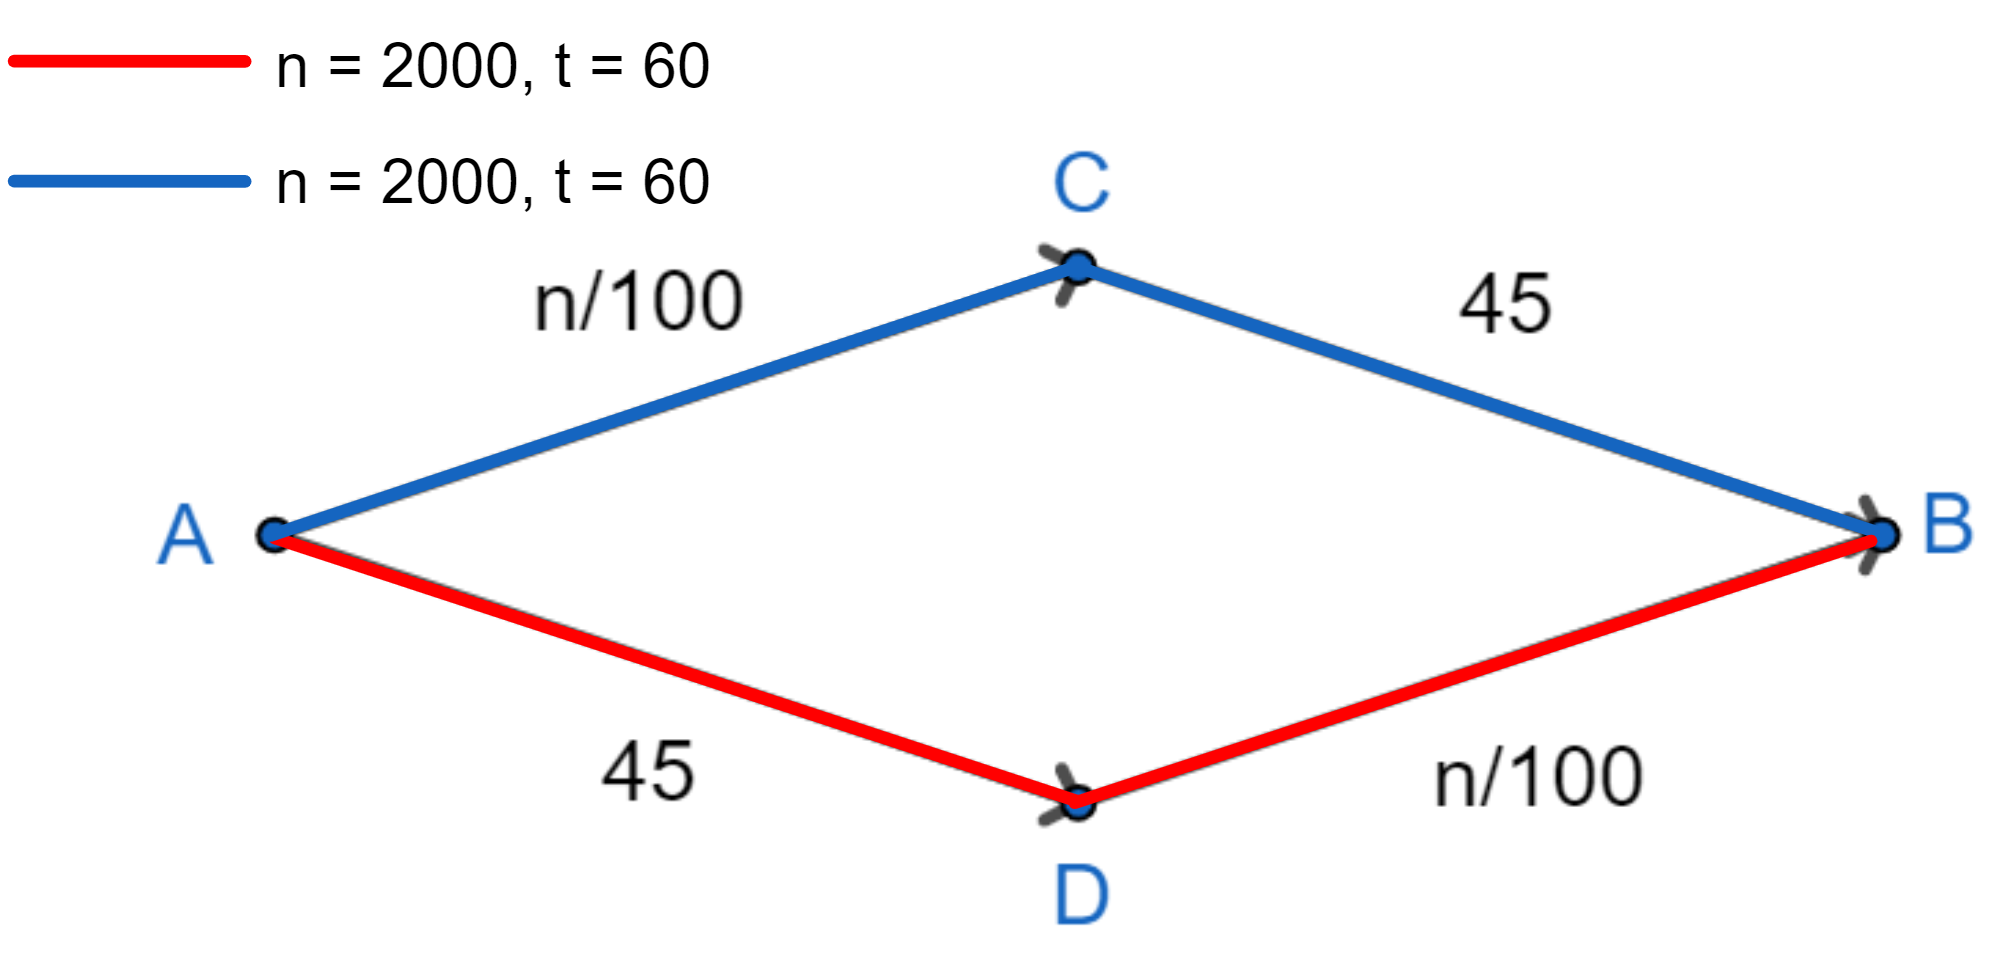
\includegraphics[width=1\linewidth]{imgs/before_braess_short.png}
				\caption{Оптимальное равновесие Нэша.\newline}
				\label{ris:braess_1}
			\end{minipage}
			\hfill
			\begin{minipage}[h]{0.45\linewidth}
				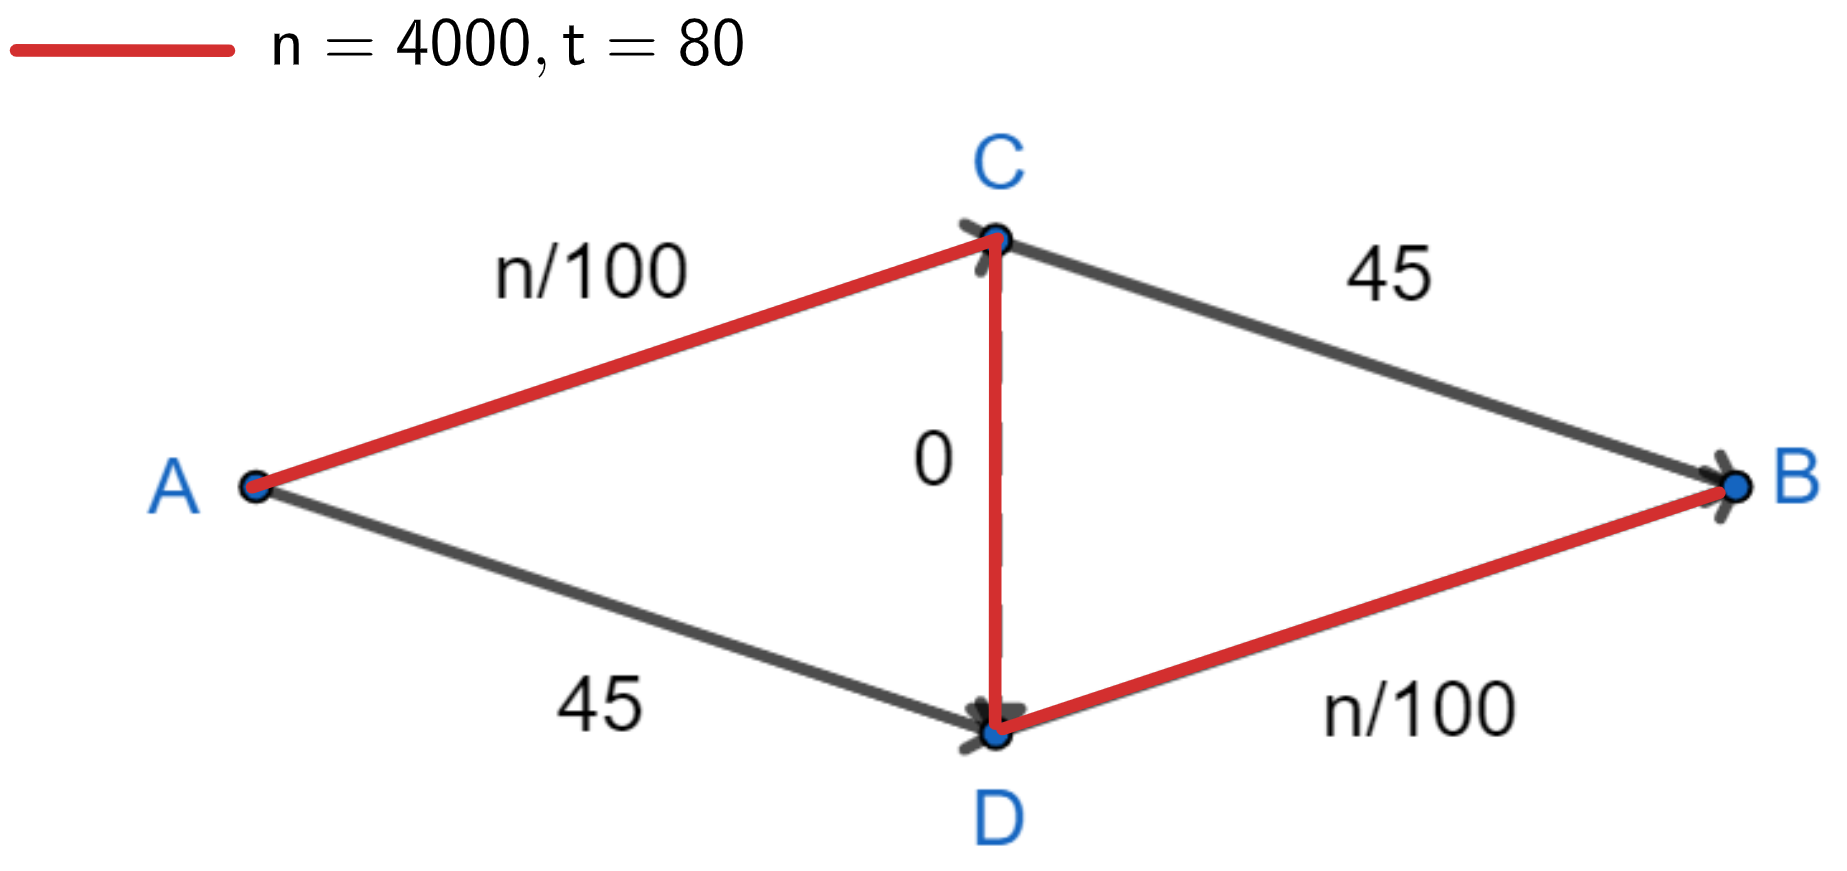
\includegraphics[width=1\linewidth]{imgs/after_braess_short.png}
				\caption{Неоптимальное равновесие Нэша с ребром CD}
				\label{ris:braess_2}
			\end{minipage}
		\end{center}
	\end{figure}
	
\end{frame}

\begin{frame}\frametitle{Парадокс Браеса}
	Оптимальное среднее время в пути достигается, когда группы участников не влияют друг на друга.
	\begin{figure}[H]
	\begin{center}
		\begin{minipage}[h]{0.60\linewidth}
			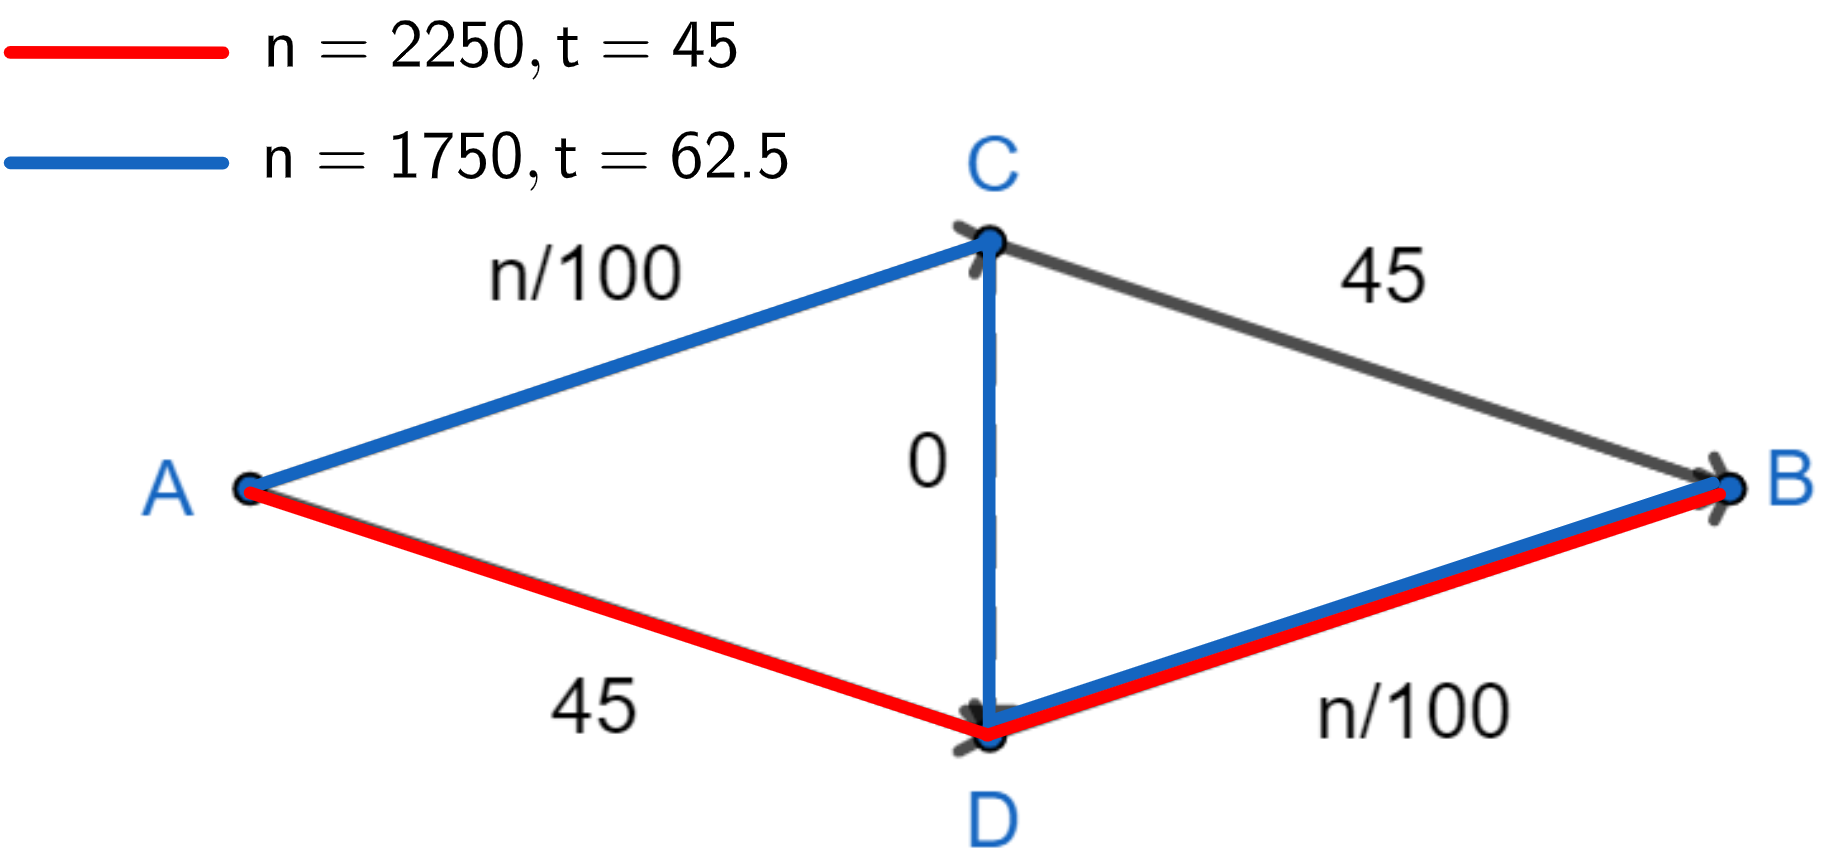
\includegraphics[width=1\linewidth]{imgs/braess_after_opt_short.png}
			\caption{Оптимальное равновесие Нэша с ребром CD}
			\label{ris:braess_3}
		\end{minipage}
	\end{center}
\end{figure}
\end{frame}

\begin{frame}\frametitle{История описания транспортного потока}
	Некооперативная игра на основе экономической модели (1952):
	\begin{itemize}
		\item Выигрыш --- затраты на маршрут.
		
		\item Затраты зависят от суммарной величины потока по пути. 
	\end{itemize}

	\bigskip

	Сжимаемая жидкость в гидродинамической модели (1955):
	\begin{itemize}
		\item Выполняется закон сохранения массы.
		
		\item Есть соответствие между скоростью и плотностью потока.
	\end{itemize}
\end{frame}

\begin{frame}\frametitle{История описания транспортного потока}
	Моделирование однополосного движения (1959):
	\begin{itemize}
		\item Учитывается порядок участников на полосе.
		
		\item Скорость участника зависит от состояния (положения и скорости) впереди идущих участников.
	\end{itemize}

	\bigskip
	
	Модель клеточных автоматов (1986):
	\begin{itemize}
		\item Дорога разбивается на клетки.
		
		\item Движение происходит в дискретном времени.
		
		\item Присутствуют случайные возмущения движения.
	\end{itemize}
\end{frame}

\begin{frame}\frametitle{Неформальная постановка задачи}
	
	Поставим задачу следующим образом:
	
	\begin{itemize}
		\item Считаем, что заданы законы изменения скорости участников при их взаимодействии друг с другом.
		 %Считаем, что задана модель движения, по которой восстанавливается движение всех участников.
		
		\item Оптимизируем некоторую общую функцию временных затрат, зависящую только от временных затрат каждого участника.
	\end{itemize}
	\bigskip
	Сложность: область оптимизации есть множество всевозможных комбинаций путей.
	
	\bigskip
	
	Новизна подхода заключается в следующем:
	\begin{itemize}
		\item Необходимо построить оптимальные маршруты для всех участников.
		
		\item Каждый участник индивидуален и не является частью потока.
	\end{itemize}

	\bigskip

	%В реальных условиях невозможно управлять всеми транспортами дорожной сети, поэтому в такой постановке задача никогда не рассматривалась.

\end{frame}

\section{Постановка задачи}

\begin{frame}\frametitle{Основные определения}
  \begin{itemize}
	\item   \emph{Дорожной сетью} назовем тройку $G = (V, E, l)$, где $(V, E)$ --- ориентированный граф с длинами ребер $l: E \rightarrow \mathbb{R}_{>0} $.
	
	\item Предположим, что имеется $n$ участников с заданными точками отправления $A_i \in V$ и прибытия $B_i \in V$. Пусть множество $P_i$ есть множество всех простых путей из $A_i$ в $B_i$. Элемент декартового произведения ${P = \prod \limits_{i = 1} ^ n P_i}$ назовем \emph{комбинацией путей}.
	
	\item Пусть известно, что при комбинации путей участников $\textbf{p} = \left(p_1, \ldots, p_n\right)\in P$ $i$-ый участник затрачивает $T_i(\textbf{p}) \in \mathbb{R}_{\ge 0}$ времени на свой путь.  Функции $T_i$ назовем \textit{функциями временных затрат} участника $i$.
	
	\item \textit{Некооперативным прокладыванием пути} назовем пятерку $F=(n, G, \{A_i\}_{i = 1}^{n}, \{B_i\}_{i = 1}^{n}, \{T_i\}_{i = 1}^{n})$.
\end{itemize}
\end{frame}

\begin{frame}\frametitle{Общая постановка задачи}
 
  	
    Функцию $\Phi (\textbf{p}) = \phi (T_1 (\textbf{p}), \ldots, T_n(\textbf{p}))$, определенную на множестве всех возможных комбинаций путей $P$ и отображающую его во множество действительных чисел назовем \textit{функцией стоимости}.
  	\begin{enumerate}
  		\item  $\Phi (\textbf{p}) = \frac{1}{n}\sum\limits_{i = 1}^n T_i (\textbf{p})$ --- средние временные затраты. 
  		\item  $\Phi (\textbf{p}) = \frac{1}{|I|}\sum\limits_{i \in I} T_i (\textbf{p})$ --- приоритетные временные затраты.
  		\item  $\Phi (\textbf{p}) = \max\limits_{i = 1, \ldots, n} T_i (\textbf{p})$ --- максимальные временные затраты.
  	\end{enumerate}
  
  	\bigskip
	Для заданных некооперативного прокладывания пути $F$ и функции стоимости $\Phi$ необходимо найти комбинацию путей $\textbf{p}^*$ такую, что функция стоимости на ней минимальна, то есть
	\begin{equation}
		\Phi (\textbf{p}^*) = \minn\limits_{ \textbf{p} \in P} \Phi (\textbf{p}).
	\end{equation}
  	
\end{frame}

\begin{frame}\frametitle{Постановка задачи в терминах модели движения}
\textit{Моделью движения} назовем набор положительных отделенных от нуля ограниченных функций $\{v_i(\textbf{p}, t)\}_{i = 1}^n$.

\begin{theorem}
	Для заданной модели движения $\{v_i(\textbf{p}, t)\}_{i = 1}^n$ существует единственный набор функций $\{T_i(\textbf{p})\}_{i = 1}^n$, описыващий время прибытия участника $i$.
\end{theorem}

Поиск таких функций называется \textit{моделированием движения}.

\bigskip

Для заданных модели движения $\{v_i(\textbf{p}, t)\}_{i = 1}^n$, некооперативного прокладывания пути $F$, в котором функции временных затрат получены путем моделирования движения, и функции стоимости $\Phi$ необходимо найти комбинацию путей $\textbf{p}^*$ такую, что функция стоимости на ней минимальна.

\end{frame}

\begin{frame}\frametitle{Постановка задачи в терминах модели движения}
	Значения функции $v_i(\textbf{p}, t)$ могут быть посчитаны применением правил движения в момент моделирования:
	\begin{enumerate}
		\item Тормозим, если впереди идущий слишком близко к нам.
		\item Ускоряемся, если впереди идущий достаточно далеко от нас.
		\item Не превышаем скорость.
		\item Тормозим перед поворотами.
	\end{enumerate}
\end{frame}

\section{Решение задачи}

\begin{frame}\frametitle{Макроскопические модели движения}
	Модель движения назовем \textit{макроскопической}, если скорость каждого участника зависит от загруженности ребра, на котором он движется.

	\begin{theorem}
	Пусть модель движения $ v_i(\textbf{p}, t)$ макроскопическая и функция затрат $\phi$ --- линейная. Тогда задача поиска оптимальной комбинации путей есть задача смешанного целочисленного линейного программирования.
	\end{theorem}
\end{frame}

\begin{frame}\frametitle{Микроскопические модели движения}
	 Модель движения назовем \textit{микроскопической}, если она не является макроскопической.
	
	\bigskip
	Примеры микроскопических моделей:
	\begin{itemize}
		\item \textit{Модель пропорциональной скорости}
		\begin{equation}
			\label{eq:micro}
			v_i(t)=
			\begin{cases}
				v_{max}, & i = n,
				\\
				v_{max} \frac{d_i(t)}{D} ,& i \ne n,
			\end{cases}
		\end{equation}
	где $v_{max}$ --- максимальная скорость, $D$ --- расстояние взаимодействия, а $d_i(t)$ --- расстояние до следующего участника.
	
	\item \textit{Модель снижения скорости}
	\begin{equation}
		v_{n - k} = v_{max} - c_n k, \; k = 0, \dots, n - 1,
	\end{equation}
	где $v_{max}$ --- максимальная скорость, $c_n$ --- величина снижения скорости.
	
	\end{itemize}
\end{frame}

\begin{frame}\frametitle{Кооперативное равновесие и алгоритмы его поиска.}
\textit{Кооперативным равновесием} некооперативного прокладывания пути $F$ и функции стоимости $\Phi (\textbf{p})$ назовем комбинацию путей $\widetilde{\textbf{p}} \in P$, которая является равновесием Нэша некооперативной игры $\widetilde{\Gamma} = (n, \{P_i\}_{i = 1}^n, \{-\Phi\}_{i = 1}^n)$.

Оптимальное решение является кооперативным равновесием.

\bigskip
Алгоритмы поиска кооперативного равновесия:
\begin{itemize}
	\item \textit{Поиск неподвижной точки}: последовательно решаем задачу оптимизации по каждому из путей, пока это возможно. 
	\item  \textit{Алгоритм последовательного добавления участников}: будем добавлять в нашу задачу по одному участнику и сводить их к неподвижной точке.
\end{itemize}
\end{frame}

\section{Практические Результаты}
\begin{frame}\frametitle{Одинаковый приоритет участников}
Исследуем движение $n = 30$ участников в графе путем поиска кооперативных равновесий для функции стоимости $\phi(T_1, \ldots, T_n) = \frac{1}{n}\sum\limits_{i = 1}^n T_i$.
\begin{figure}[H]
	\begin{center}
		\begin{minipage}[h]{0.35\linewidth}
			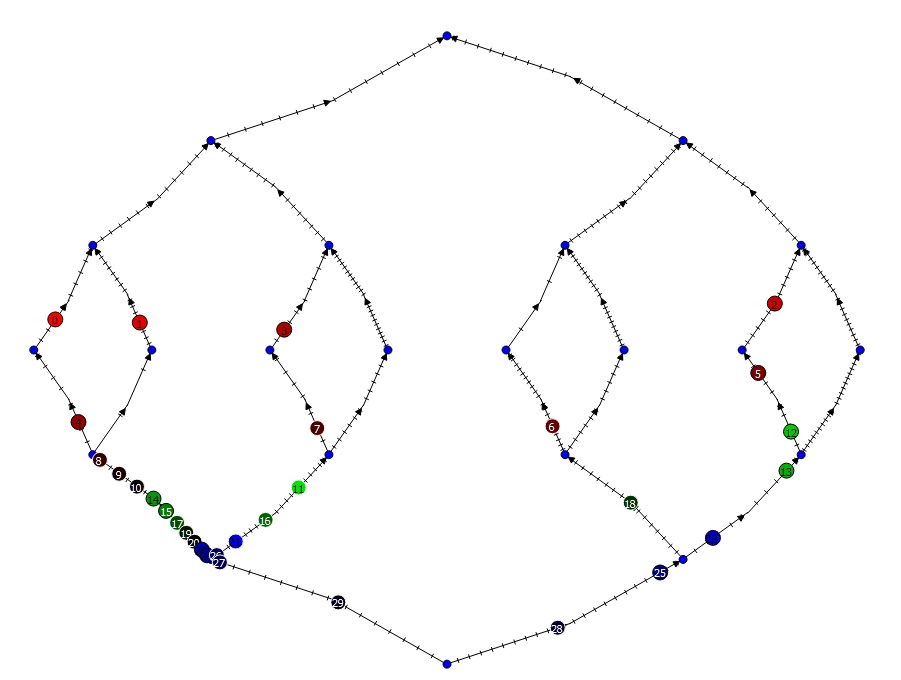
\includegraphics[width=1\linewidth]{imgs/average_good.jpg}
			\caption{Результат минимизации затрат, $\Phi(\widetilde{\textbf{p}}) = 1063$.}
		\end{minipage}
		\hfill
		\begin{minipage}[h]{0.35\linewidth}
			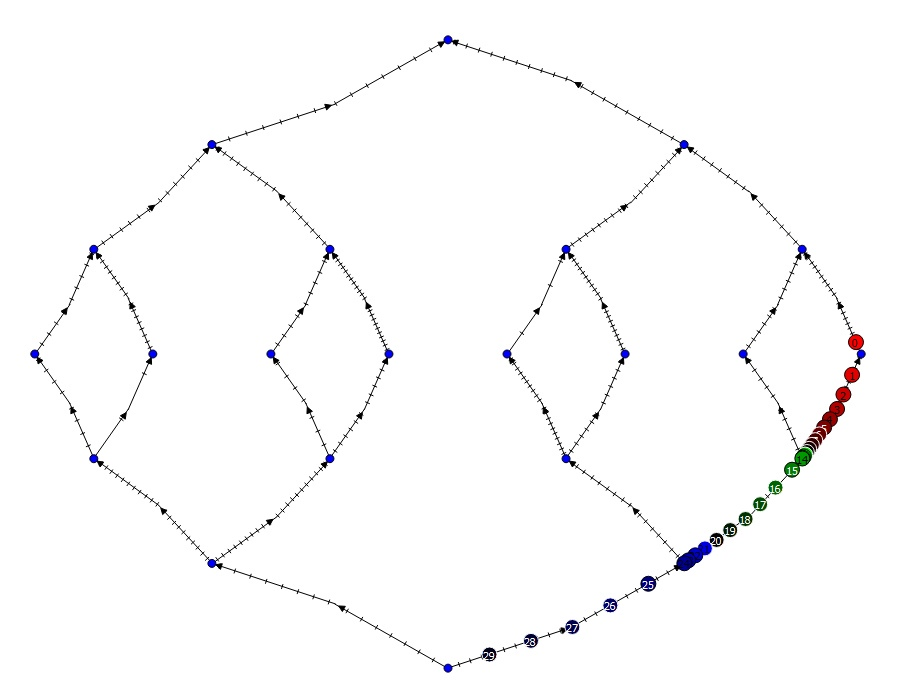
\includegraphics[width=1.\linewidth]{imgs/average_bad.jpg}
			\caption{Результат максимизации затрат, $\Phi(\widetilde{\textbf{p}}) = 1576$.}
		\end{minipage}
	\end{center}
\end{figure}

\begin{itemize}
	\item Результат соответствует ожиданиям.
	\item Результат может быть неоптимальным.
\end{itemize}

\end{frame}


\begin{frame}\frametitle{Поиск путей для приоритетных участников}
Исследуем движение $n = 30$ участников в графе путем поиска кооперативных равновесий для функции стоимости $\phi(T_1, \ldots, T_n) = \frac{1}{3} \left(T_1 + T_{\frac{n}{2}} + T_n\right)$.
\begin{figure}[H]
	\begin{center}
		\begin{minipage}[h]{0.35\linewidth}
			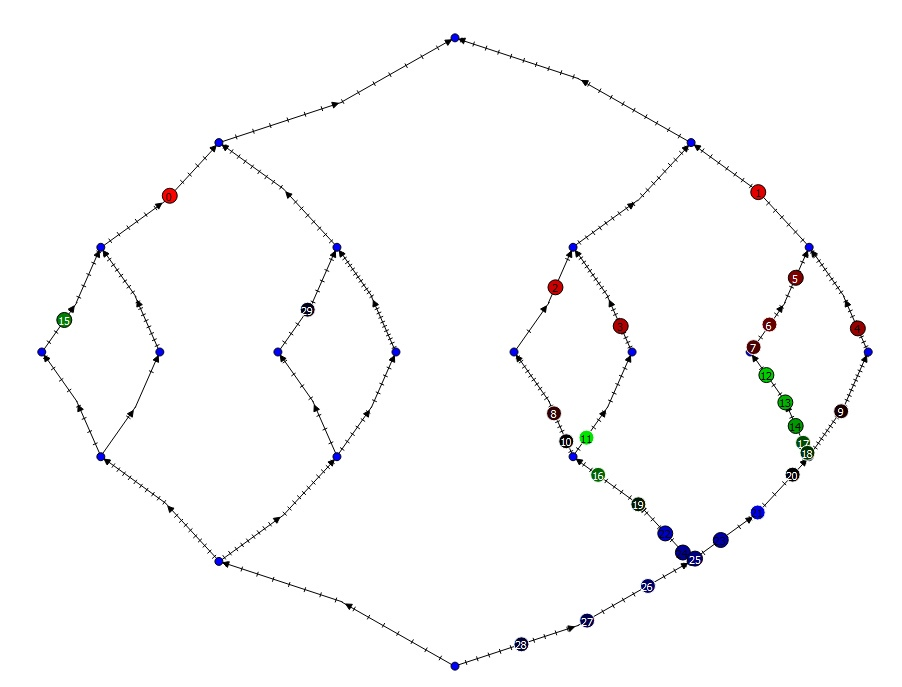
\includegraphics[width=1\linewidth]{imgs/prior_good.jpg}
			\caption{Результат минимизации затрат, $\Phi(\widetilde{\textbf{p}}) = 778.34$.}
		\end{minipage}
		\hfill
		\begin{minipage}[h]{0.35\linewidth}
			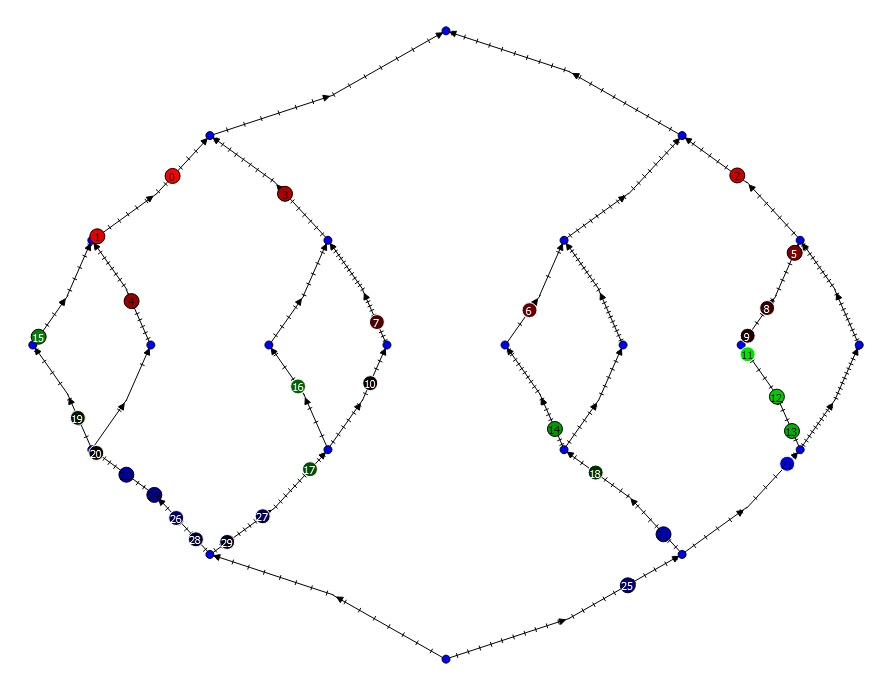
\includegraphics[width=1\linewidth]{imgs/prior_bad.jpg}
			\caption{Результат минимизации затрат, $\Phi(\widetilde{\textbf{p}}) = 950.37$.}
		\end{minipage}
	\end{center}
\end{figure}

\begin{itemize}
	\item Результат зависит от начального распределения путей.
	\item Результат может быть неоптимальным.
\end{itemize}

\end{frame}

\begin{frame}\frametitle{Заключение}
	\begin{itemize}
		\item Предложено описание общего принципа взаимодействия участников, заключающегося в задании некоторой модели движения.
		\item Разработан и реализован алгоритм моделирования движения в соответствии с заданной моделью движения.
		\item Выделен класс моделей, для которого доказана возможность сведения поставленной задачи к задаче смешанного целочисленного линейного программирования.
		\item Разработаны и реализованы алгоритмы поиска кооперативного равновесия.
		\item Разработано ПО для моделирования, поиска оптимального пути и оптимальной комбинации путей в произвольной модели движения.
	\end{itemize}
\end{frame}

\end{document}
